\begin{frame}
  \frametitle{The discontinuous Galerkin (DG) method uses
  discontinuous basis functions}
  \begin{columns}
    \begin{column}{0.3\textwidth}
      \only<1>{
      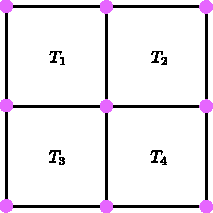
\includegraphics[width=1.0\textwidth]{pdf/box-mesh-before-split.pdf}
    }
    \only<2->{
      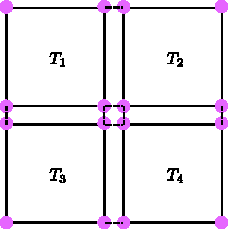
\includegraphics[width=1.0\textwidth]{pdf/box-mesh-after-split.pdf}
    }
    \end{column}
    \begin{column}{0.7\textwidth}
      \only<1-2>{
    \def\svgwidth{1.0\textwidth}
    \import{pdf/}{lin.pdf_tex}
  }
      \only<3->{
    \def\svgwidth{1.0\textwidth}
    \import{pdf/}{lin-dg.pdf_tex}
  }
    \end{column}
  \end{columns}
  \hspace{2em}
  \begin{equation*}
    V_h = P^k(\mcT_h) = \{ v_h \in L^2(\Omega): v_h|_{T} \in P^k(T)\; \foralls T \in
    \mcT_h\} 
  \end{equation*}
\end{frame}
